% Created 2022-07-20 mer. 21:17
% Intended LaTeX compiler: pdflatex
\documentclass[10pt,table,dvipsnames,compress]{beamer}
\usepackage[utf8]{inputenc}
\usepackage[T1]{fontenc}
\usepackage{graphicx}
\usepackage{longtable}
\usepackage{wrapfig}
\usepackage{rotating}
\usepackage[normalem]{ulem}
\usepackage{amsmath}
\usepackage{amssymb}
\usepackage{capt-of}
\usepackage{hyperref}
\usetheme{default}
\useinnertheme{rounded}
\useoutertheme[subsection=false]{miniframes}
\date{}
\title{\texttt{riskmapjnr} Python package for mapping the deforestation risk using JNR's methodology}
\title[riskmapjnr]{\texttt{riskmapjnr} Python package for mapping the deforestation risk using JNR's methodology}
\usepackage{lmodern}
\usepackage{pgf}
\usepackage{color}
\usepackage[english,french]{babel}
\definecolor{vertmoyen}{RGB}{51,110,23} % vert moyen
\definecolor{blueFRB}{HTML}{31859c}
\usecolortheme[named=blueFRB]{structure}
\usepackage{tabularx} % varier la largeur du tableau
\usepackage{layout}
\setlength{\LTleft}{-5cm plus 1 fill}
\setlength{\LTright}{-5cm plus 1 fill}
\usepackage{booktabs}
\usepackage{arydshln} %% dashlines for tabular
\newcommand{\logit}{\text{logit}}
\newcommand{\bs}[1]{\boldsymbol{#1}}
\newcommand{\R}{\textnormal{\sffamily\bfseries R}}
\newcommand{\pkg}[1]{{\fontseries{b}\selectfont #1}}
\newcolumntype{C}[1]{>{\centering\arraybackslash}m{#1}}

\setbeamertemplate{footline}[frame number]
\setbeamertemplate{frametitle}{%
\usebeamerfont{frametitle}\insertframetitle%
\vphantom{g} % To avoid fluctuations per frame
\par
\centering 
\includegraphics[width=\textwidth]{figs/Barre_couleur}
}
\beamertemplatenavigationsymbolsempty

% Logo
\newif\ifplacelogo % create a new conditional
\logo{\ifplacelogo
\includegraphics[width=0.5\textwidth]{figs/partners_logos}\fi}

%Call table of contents at the beginning of each section
\AtBeginSection[]{
\placelogotrue
\begin{frame}
\frametitle{Plan}
\begin{columns}[c]
\begin{column}{0.5\textwidth}
\tableofcontents[sections=1,currentsection]
\vspace{0.5cm}
\tableofcontents[sections=2,currentsection]
\end{column}
\begin{column}{0.5\textwidth}
\tableofcontents[sections=3,currentsection]
\vspace{0.5cm}
\tableofcontents[sections=4,currentsection]
\end{column}
\end{columns}
\end{frame}
\placelogofalse
}

\AtBeginSubsection[]{}

\hypersetup{
colorlinks=true,
linkcolor=Black,
filecolor=Maroon,
citecolor=Blue,
urlcolor=Maroon}

% Disable monospaced font for URLs
\urlstyle{same}

\hypersetup{
 pdfauthor={Ghislain Vieilledent},
 pdftitle={\texttt{riskmapjnr} Python package for mapping the deforestation risk using JNR's methodology},
 pdfkeywords={},
 pdfsubject={},
 pdfcreator={Emacs 27.1 (Org mode 9.5.3)}, 
 pdflang={English}}
\begin{document}


% Title page
{
  \setbeamertemplate{navigation symbols}{}
  \begin{frame}[plain, noframenumbering]
  
  \begin{center}
  \small{\textbf{FAO -- IMPRESS project -- July 2022}}
  \end{center}
  \vspace{-1cm}
  \titlepage % Presentation first page
  \vspace{-3.5cm}
  \begin{center}
    
\includegraphics[width=\textwidth]{figs/Barre_couleur}\\
    \vspace{0.5cm}
    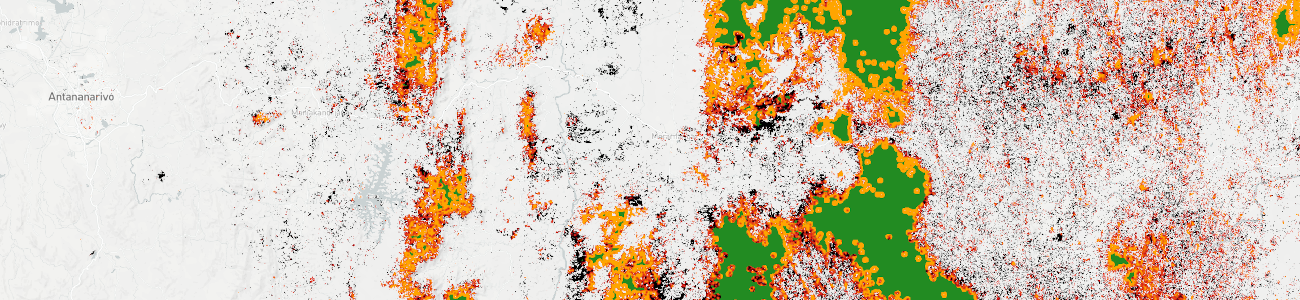
\includegraphics[width=10cm]{figs/riskmapjnr-example}\\
    \vspace{0.3cm}
    \small{Ghislain VIEILLEDENT$^{1}$\hspace{0.25cm}Pierrick RAMBAUD$^{2}$\hspace{0.25cm}Rémi d'ANNUNZIO$^{2}$}\\
    \vspace{0.15cm}
    {\scriptsize
      \begin{tabular}{l}
        $[1]$ \textbf{Cirad} UMR AMAP, $[2]$ \textbf{FAO} REDD$+$ NFM
      \end{tabular}
    }\\
    \vspace{0.3cm}
    
\includegraphics[width=0.75\textwidth]{figs/partners_logos}
    
  \end{center}
  \end{frame}
}

% %%%%%%%%%%%%%%%%%%%%%%%%%%%%%%%%%%%%%%%%%%%%%%%%%%%%%%%%%%%%%%%%

\placelogotrue
\begin{frame}
  \frametitle{Plan}
  \begin{columns}[c]
    \begin{column}{0.5\textwidth}
      \tableofcontents[sections=1]
      \vspace{0.5cm}
      \tableofcontents[sections=2]
    \end{column}
    \begin{column}{0.5\textwidth}
        \tableofcontents[sections=3]
        \vspace{0.5cm}
        \tableofcontents[sections=4]
    \end{column}
  \end{columns}
\end{frame}
\placelogofalse

\section{Introduction}
\label{sec:org0a7659f}

\subsection{Context}
\label{sec:org856e0ab}

\begin{frame}[label={sec:org5c2df49}]{Context}
\begin{itemize}
\item Paris Agreement on climate change
\item REDD+: Reducing Emissions from Deforestation and forest Degradation
\item IMPRESS (Improving Measurement for Payments to Reduce Emissions and Strengthen Sinks) FAO -- UK-PACT project
\item VCS Jurisdictional and Nested REDD+ (JNR): certification of jurisdictional REDD+ programs and nested projects
\end{itemize}

\begin{center}
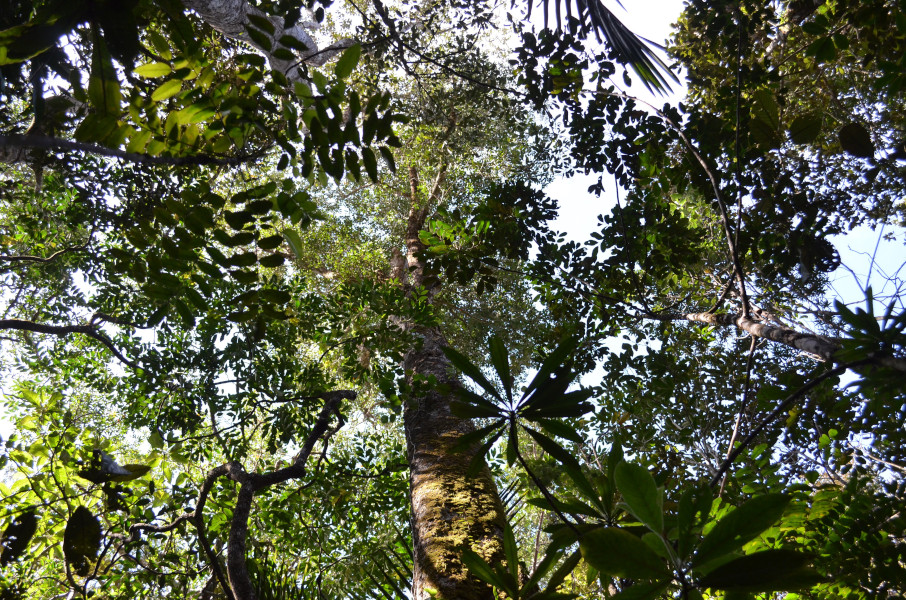
\includegraphics[width=0.5\textwidth]{figs/Canopy-NC.jpg}
\end{center}
\end{frame}

\subsection{Objectives}
\label{sec:orga3502c6}

\begin{frame}[label={sec:orgdae1938}]{Objectives}
\begin{block}{Allocate the deforestation spatially}
\begin{itemize}
\item Given a deforestation intensity (ha/yr) in a jurisdiction, how to allocate deforestation spatially? \alert{\(\Rightarrow\) Map of the deforestation risk}.
\item \href{https://verra.org/wp-content/uploads/2021/04/DRAFT\_JNR\_Risk\_Mapping\_Tool\_15APR2021.pdf}{JNR risk mapping methodology}, by Verra and CBI (Carbon Decision International).
\item Simple methodology: use only an historical forest cover change map.
\end{itemize}
\end{block}

\begin{block}{Informatic tool to derive the risk map}
\begin{itemize}
\item Develop a tool (Python package) to derive this map.
\item Following JNR methodology.
\item Port that tool to Sepal (FAO side).
\end{itemize}

\begin{center}

\includegraphics[width=0.5\textwidth]{figs/jnr.png}
\end{center}
\end{block}
\end{frame}

\section{Functionalities}
\label{sec:orge55928d}

\subsection{Python package}
\label{sec:org5a1757e}

\begin{frame}[label={sec:org496d94d},fragile]{Python package and website}
 \begin{itemize}
\item Python package: \texttt{riskmapjnr}
\item Website: \url{https://ecology.ghislainv.fr/riskmapjnr}
\item GitHub repository with open source code: \url{https://github.com/ghislainv/riskmapjnr}
\item Tutorials: see \emph{Get Started} and \emph{Articles} sections on the website
\end{itemize}

\begin{figure}[htbp]
\centering
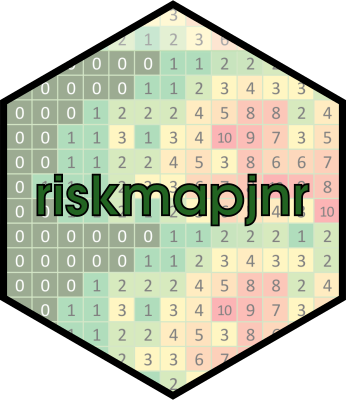
\includegraphics[width=0.25\textwidth]{figs/logo-riskmapjnr.png}
\caption{\texttt{riskmapjnr} logo}
\end{figure}
\end{frame}

\begin{frame}[label={sec:org72947a0},fragile]{Code efficiency}
 \begin{block}{Fast computations}
Python scientific libraries used:
\begin{itemize}
\item \texttt{gdal} for fast processing of georeferenced data.
\item \texttt{NumPy}, \texttt{SciPy}, and \texttt{Pandas} for fast matrix and vector operations.
\end{itemize}
\end{block}

\begin{block}{Handling large rasters}
\begin{itemize}
\item Large rasters are divided into blocks of data for in-memory processing.
\item Analysis on large geographical extents (e.g. country scale) and high spatial resolutions (eg. 30 m).
\end{itemize}
\end{block}

\begin{block}{Repeated tasks can be parallelized}
\begin{itemize}
\item Several (25 \texttimes{} 3 = 75) maps need to be produced and compared.
\item Function to produce maps on separate computer cores in parallel.
\end{itemize}
\end{block}
\end{frame}

\subsection{Functions}
\label{sec:org52bc4ec}

\begin{frame}[label={sec:org2363939},fragile]{Main functions}
 The \texttt{riskmapjnr} package includes functions to:

\begin{enumerate}
\item Estimate the distance to forest edge beyond which the deforestation risk is negligible:
\texttt{dist\_edge\_threshold()}.
\item Compute local deforestation rates using a moving window whose size can vary:
\texttt{local\_defor\_rate()}.
\item Transform local deforestation rates into categories of deforestation risks using several slicing algorithms:
\texttt{set\_defor\_cat\_zero()} and \texttt{defor\_cat()}
\item Validate maps of deforestation risk and select the map with the higher accuracy:
\texttt{defrate\_per\_cat()} and \texttt{validation()}.
\end{enumerate}
\end{frame}

\begin{frame}[label={sec:orgbfc836f},fragile]{Distance to forest edge threshold}
 \begin{itemize}
\item \texttt{rmj.dist\_edge\_threshold()}: Compute the distance to the forest edge after which the risk of deforestation becomes negligible.
\item Here, >99\% of deforestation occurs within a distance \(\le\)180m.
\item Forest pixels with a distance >180m will be in Category 0 (zero risk of deforestation).
\end{itemize}

\begin{figure}[htbp]
\centering
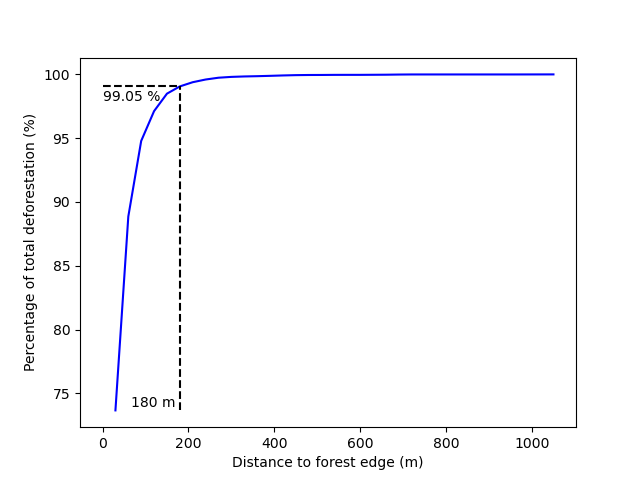
\includegraphics[width=0.5\textwidth]{figs/perc_dist.png}
\caption{\label{fig:orgf9f8f80}Cumulative deforestation as a function of the distance to forest edge.}
\end{figure}
\end{frame}

\begin{frame}[label={sec:org32c66c6},fragile]{Local deforestation rate}
 \begin{itemize}
\item \texttt{rmj.local\_defor\_rate()}: Compute a local risk of deforestation at the pixel level using a moving window made of several pixels.
\item Different window sizes can be chosen.
\item The JNR methodology recommends the use of 25 different window sizes.
\end{itemize}

\begin{figure}[htbp]
\centering
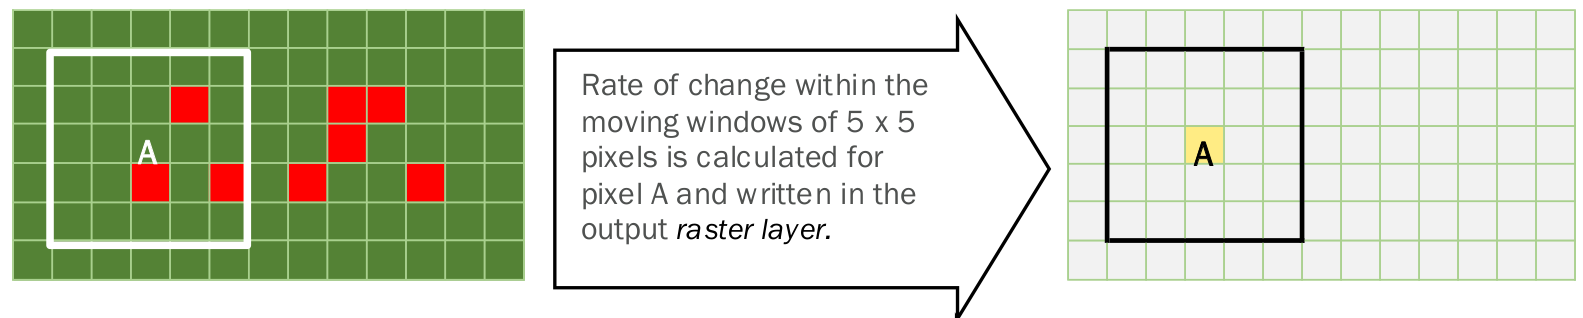
\includegraphics[width=0.8\textwidth]{figs/moving_window.png}
\caption{\label{fig:orge557364}Moving window.}
\end{figure}
\end{frame}

\begin{frame}[label={sec:org741fa91},fragile]{Categorize the deforestation risk}
 \begin{itemize}
\item \texttt{rmj.defor\_cat()}: Convert local deforestation rate into categories of deforestation risk.
\item The JNR methodology suggests to use \uline{31 categories of risk} from ``0'' to ``30'' (including the ``0'' category).
\item The JNR methodology recommends the use of \uline{three slicing algorithms}: ``equal area'', ``equal interval'', and ``natural breaks''.
\begin{itemize}
\item ``equal area'': each class covers approximately the same area
\item ``equal interval'': bins of the same range size
\item ``natural breaks'': data are normalized before applying the ``equal interval'' algorithm.
\end{itemize}
\end{itemize}

\begin{figure}[htbp]
\centering
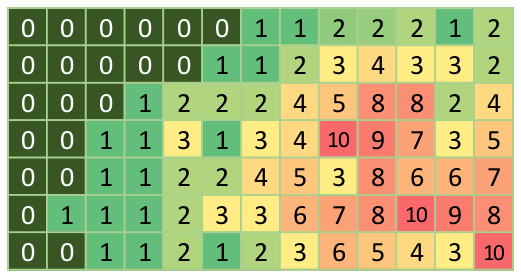
\includegraphics[width=0.4\textwidth]{figs/categories.png}
\caption{\label{fig:orgd34ebc0}Categories of deforestation risk.}
\end{figure}
\end{frame}

\begin{frame}[label={sec:org0dea292},fragile]{Validate the map}
 \begin{itemize}
\item \texttt{rmj.validation()}: Validate the map of deforestation risk on a validation period.
\item Square grid of at least 1000 spatial cells covering the jurisdiction.
\item Predicted deforestation using deforestation rates for risk categories.
\item Comparison of predictions and observations for each spatial cells
\item Accuracy index: weighted Root Mean Squared Error (wRMSE)
\end{itemize}

\begin{figure}[htbp]
\centering
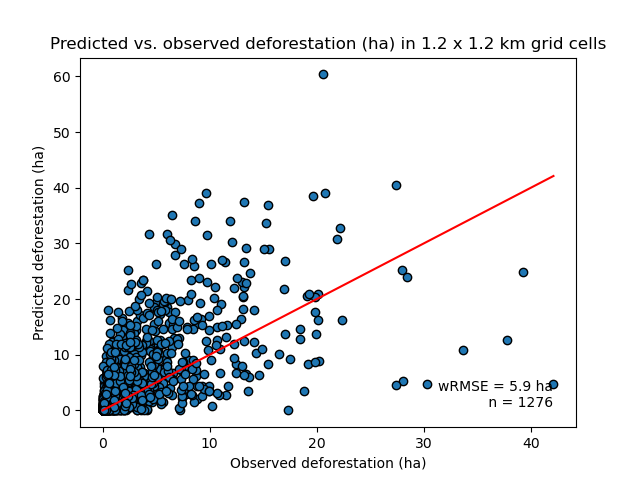
\includegraphics[width=0.5\textwidth]{figs/pred_obs_ws5_ei.png}
\caption{\label{fig:org252304e}Predictions vs. observations.}
\end{figure}
\end{frame}

\begin{frame}[label={sec:org996d16a},fragile]{Derive maps in parallel}
 \begin{itemize}
\item \texttt{rmj.makemap()}: Derive maps with different window sizes and slicing algorithms and choose the best map.
\item Maps are produced on separate computer cores in parallel.
\end{itemize}
\end{frame}

\section{Case-studies}
\label{sec:orgd0b9608}

\subsection{Jurisdictions}
\label{sec:orgc59e8b9}

\begin{frame}[label={sec:org40df261}]{Jurisdictions}
\begin{columns}
\begin{column}{0.5\columnwidth}
\begin{itemize}
\item Guadeloupe (\emph{Get Started} tutorial)
\item Madagascar tropical moist forests
\item Kenya (IMPRESS project)
\item more to come\ldots{}
\end{itemize}
\end{column}

\begin{column}{0.5\columnwidth}
\begin{figure}[htbp]
\centering
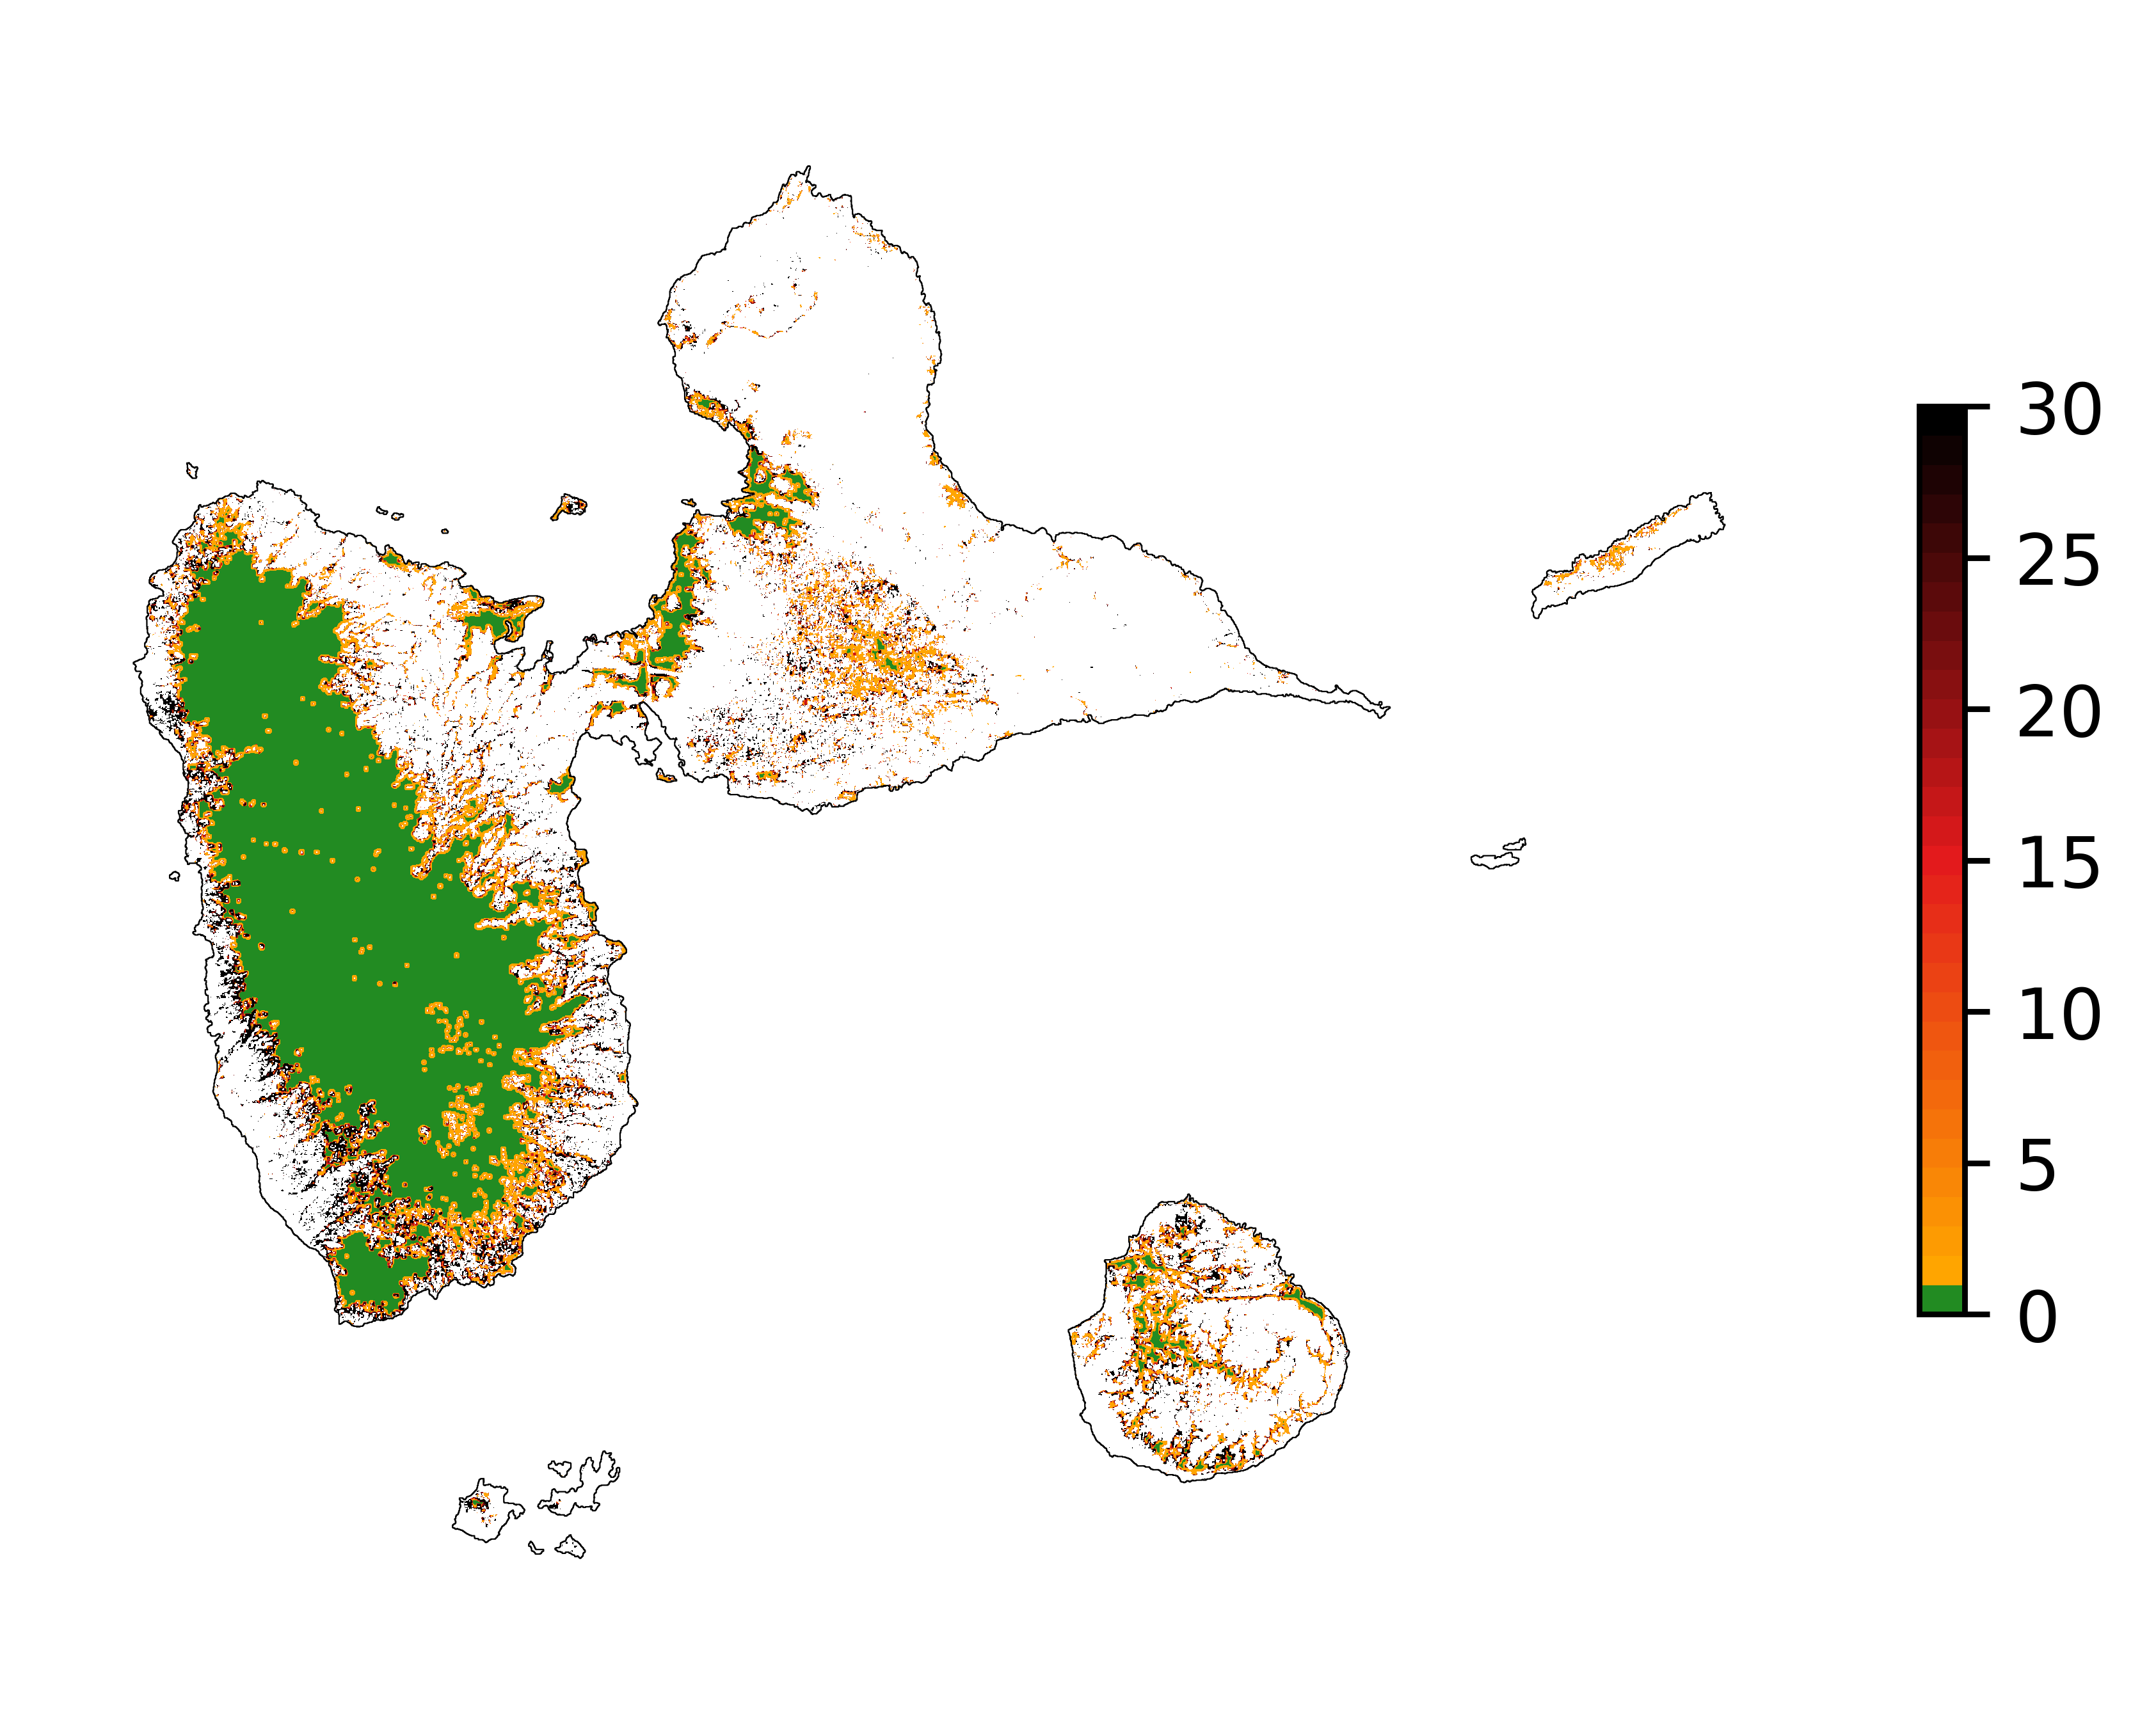
\includegraphics[width=\textwidth]{figs/riskmap_ws5_ei.png}
\caption{\label{fig:org921de52}Map of the deforestation risk for Guadeloupe.}
\end{figure}
\end{column}
\end{columns}
\end{frame}

\subsection{Kenya}
\label{sec:orgeb53768}

\begin{frame}[label={sec:org083ad31}]{Kenya}
\begin{columns}
\begin{column}{0.5\columnwidth}
\begin{itemize}
\item Forest cover change map: 2010--2014--2018.
\item Distance to forest edge threshold: 780 m.
\item Computation time: \(\sim\)20 min for 8 window sizes and 2 slicing algorithms on a personal computer using 6 cores.
\end{itemize}
\end{column}

\begin{column}{0.5\columnwidth}
\begin{figure}[htbp]
\centering
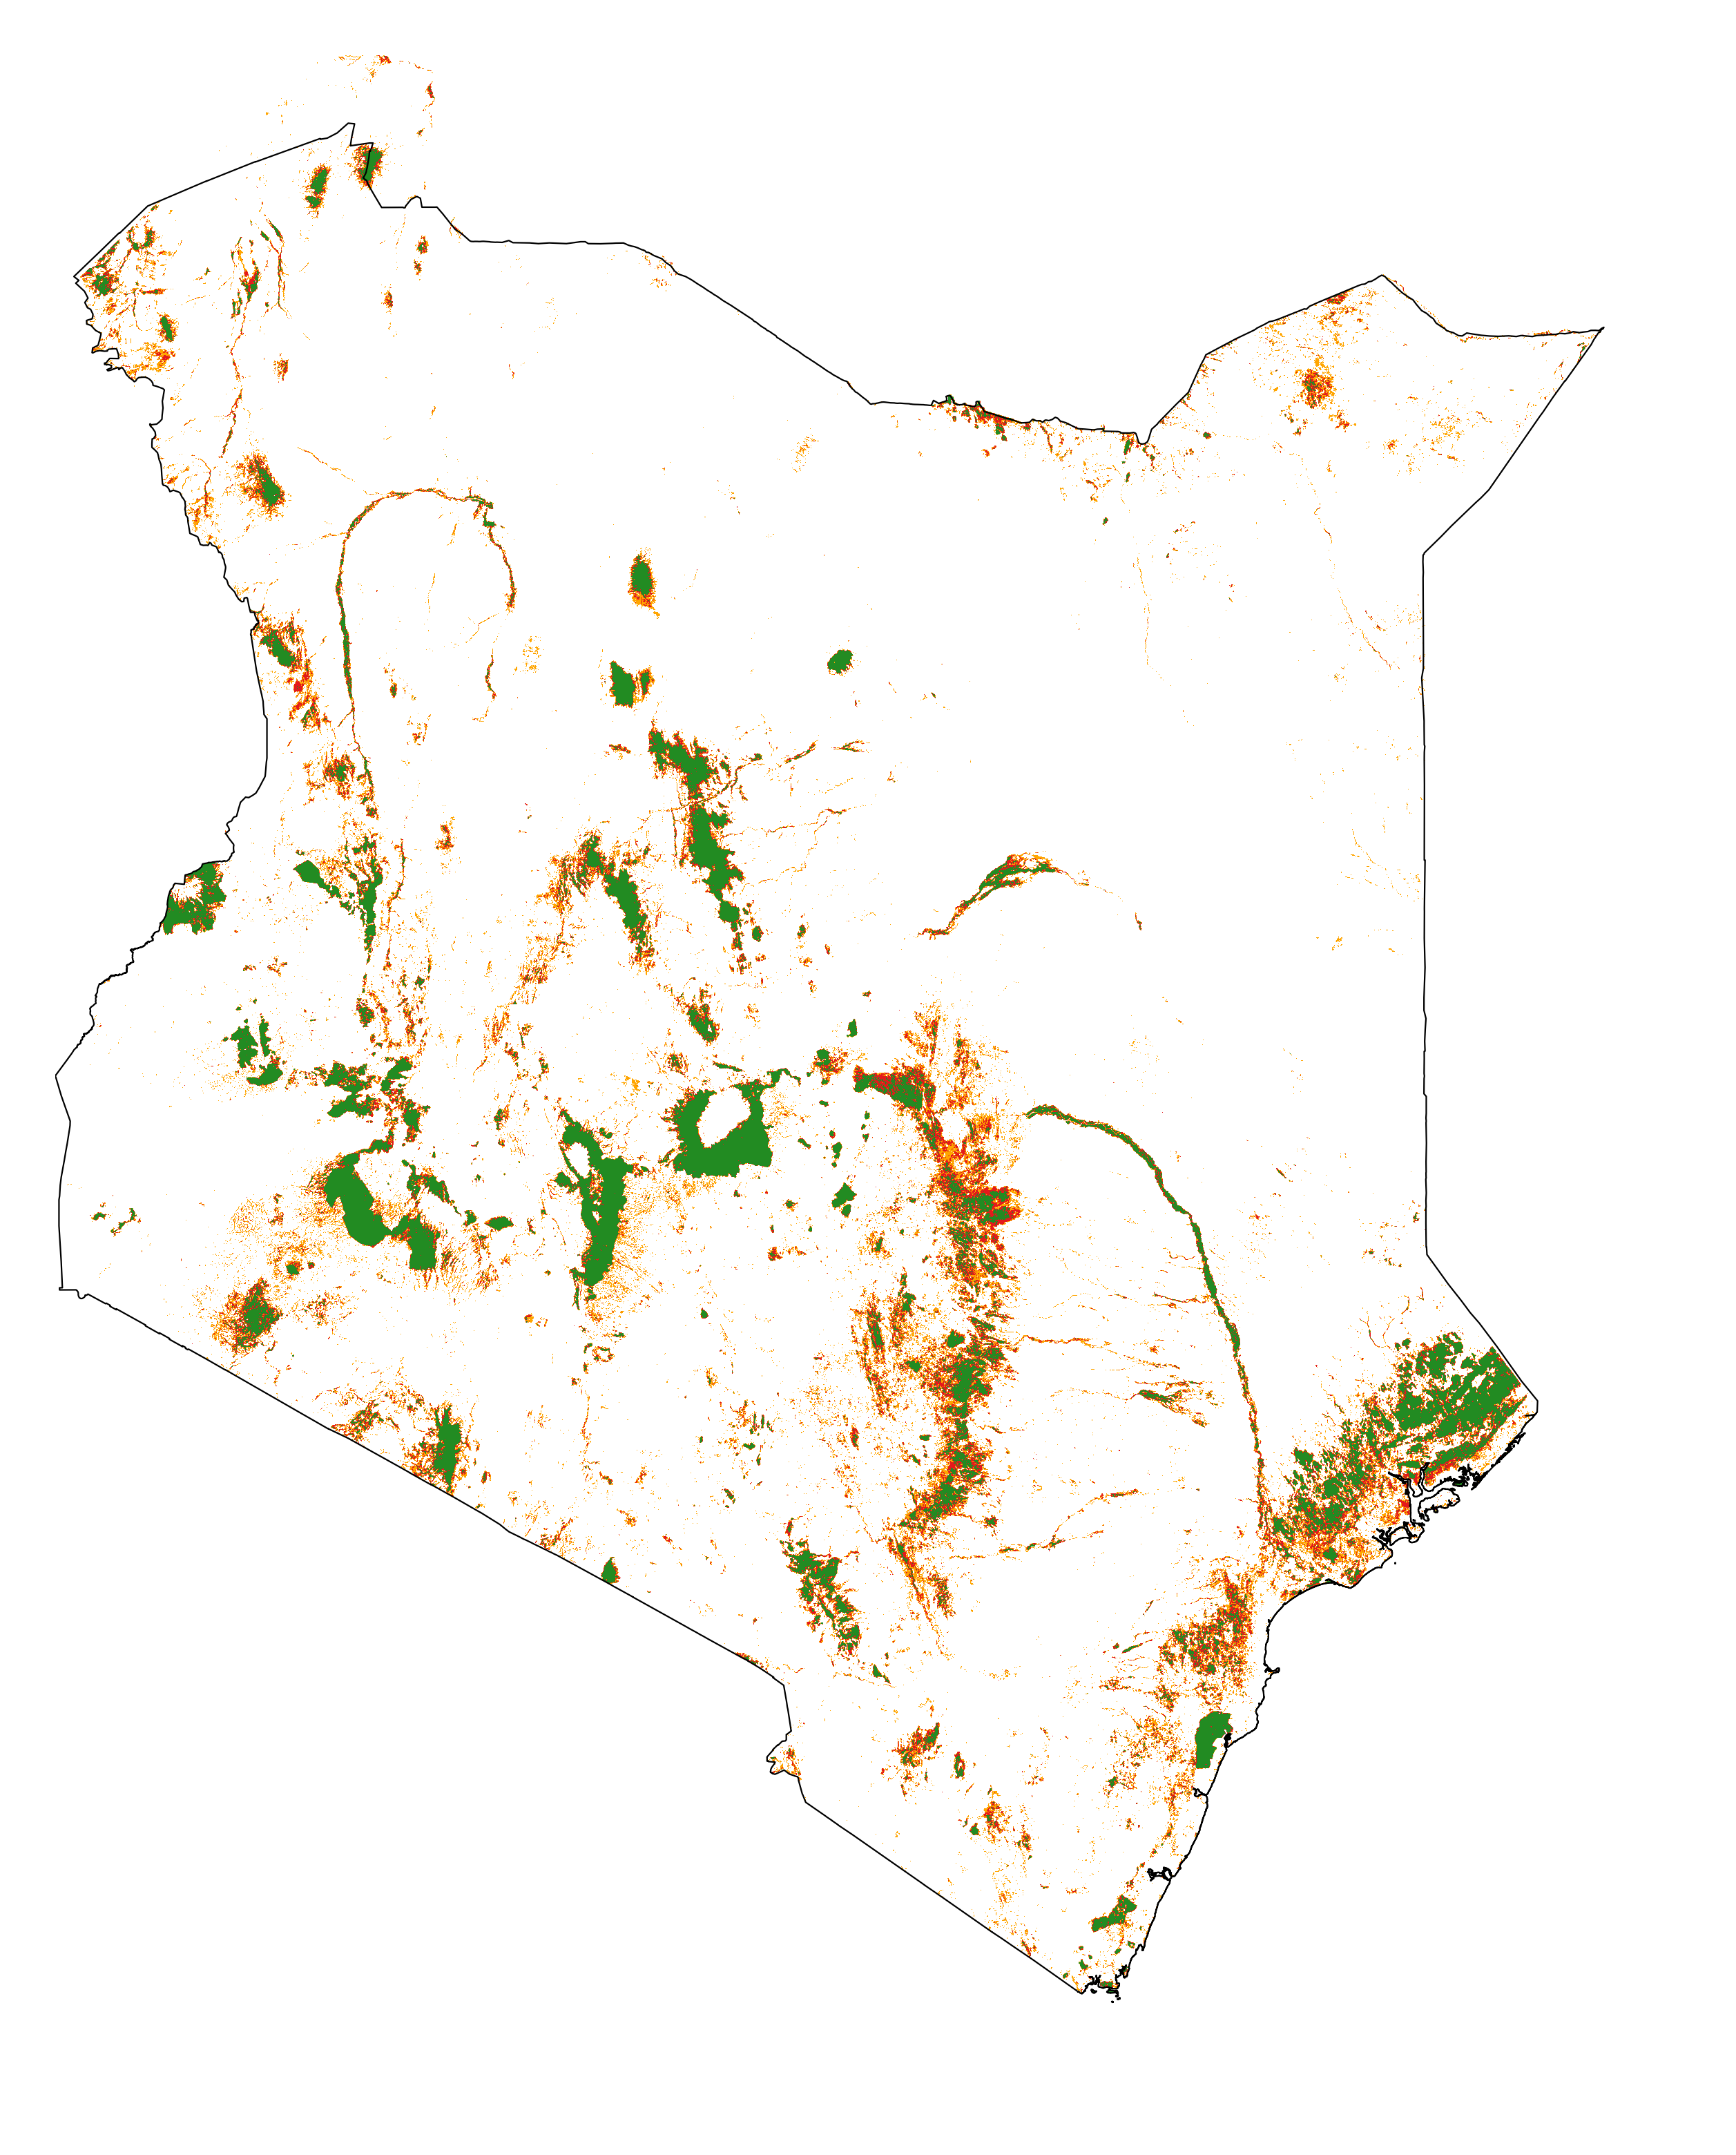
\includegraphics[width=0.9\textwidth]{figs/fcc123_kenya.png}
\caption{Forest cover change (2010--2014--2018) for Kenya.}
\end{figure}
\end{column}
\end{columns}
\end{frame}

\begin{frame}[label={sec:orgff0d72b}]{Kenya}
\begin{figure}[htbp]
\centering
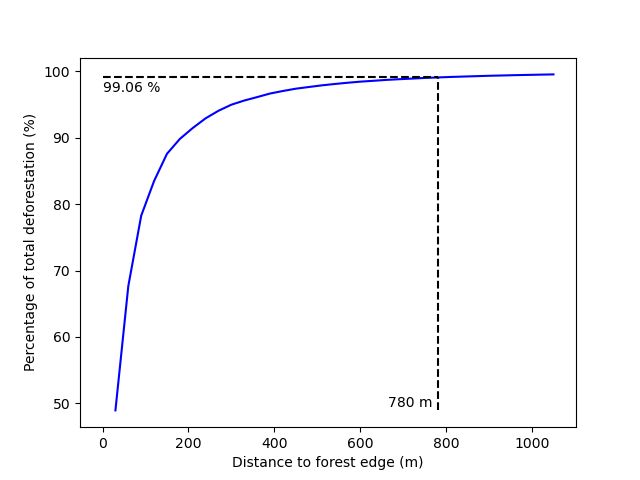
\includegraphics[width=0.6\textwidth]{figs/perc_dist_kenya.png}
\caption{Cumulative deforestation as a function of the distance to forest edge for Kenya.}
\end{figure}
\end{frame}

\begin{frame}[label={sec:orgaac6436}]{Kenya}
\begin{figure}[htbp]
\centering
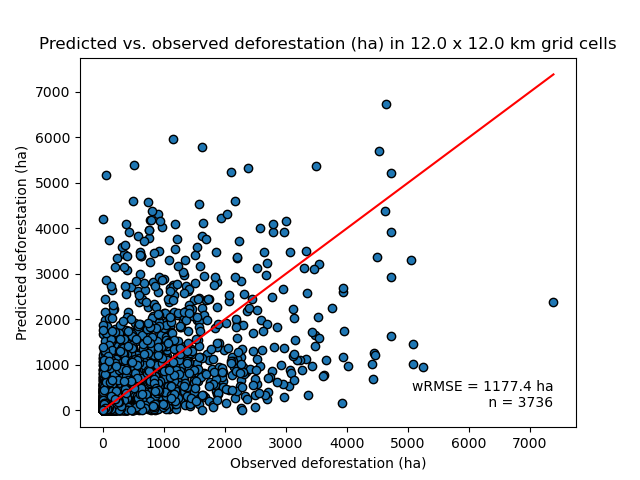
\includegraphics[width=0.6\textwidth]{figs/pred_obs_kenya.png}
\caption{Predictions vs. observations for Kenya.}
\end{figure}
\end{frame}

\begin{frame}[label={sec:orgdb50a26}]{Kenya}
\begin{figure}[htbp]
\centering
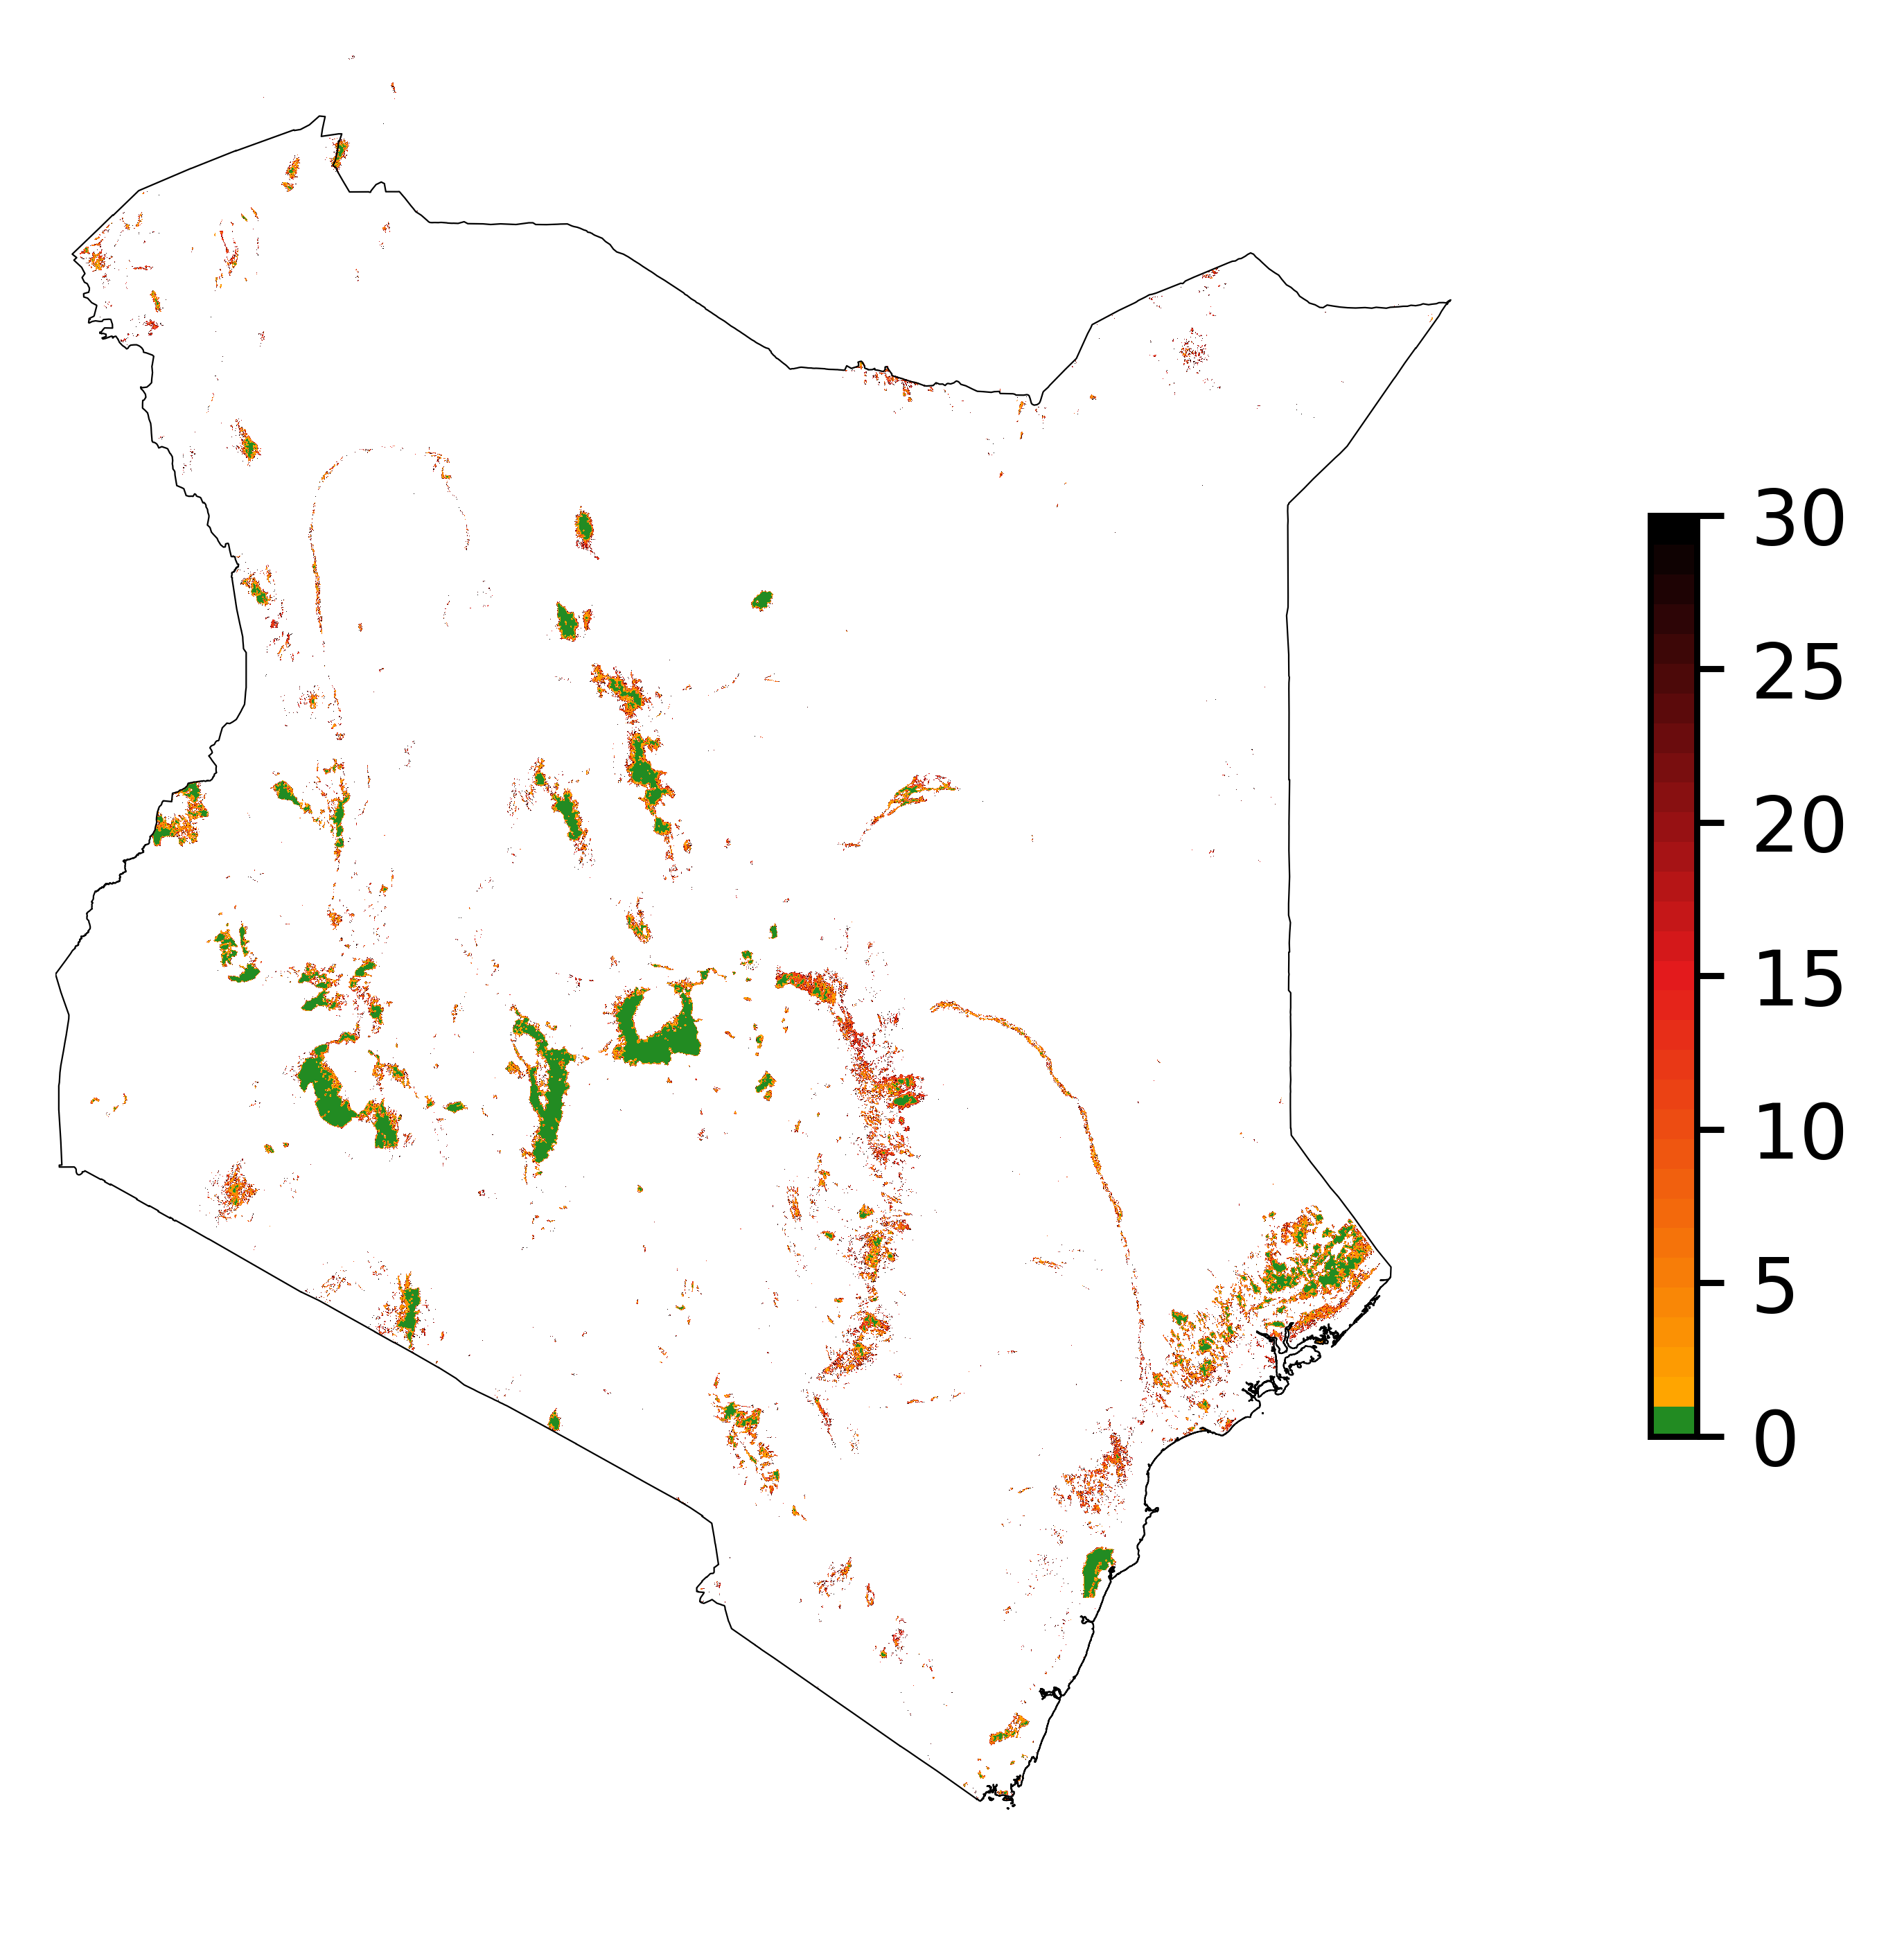
\includegraphics[width=0.6\textwidth]{figs/riskmap_kenya.png}
\caption{Map of the deforestation risk for Kenya.}
\end{figure}
\end{frame}

\section{Perspectives}
\label{sec:org4f93844}

\subsection{Comments}
\label{sec:org223b2fb}

\begin{frame}[label={sec:orgc887f58}]{Additional tests}
\begin{itemize}
\item \alert{!! First results}
\item Code might include some errors
\item Functions still need to be thoroughly tested
\item Results must be consolidated
\end{itemize}
\end{frame}

\begin{frame}[label={sec:org54ca8f7}]{Issues}
\begin{columns}
\begin{column}{0.5\columnwidth}
\begin{itemize}
\item The best window size is always the smallest.
\item No differences between slicing algorithms (ei or ea).
\item ei: ``equal interval''\\
ea: ``equal area''.
\item The ``natural breaks'' algorithm is not yet implemented.
\end{itemize}
\end{column}

\begin{column}{0.5\columnwidth}
\begin{figure}[htbp]
\centering
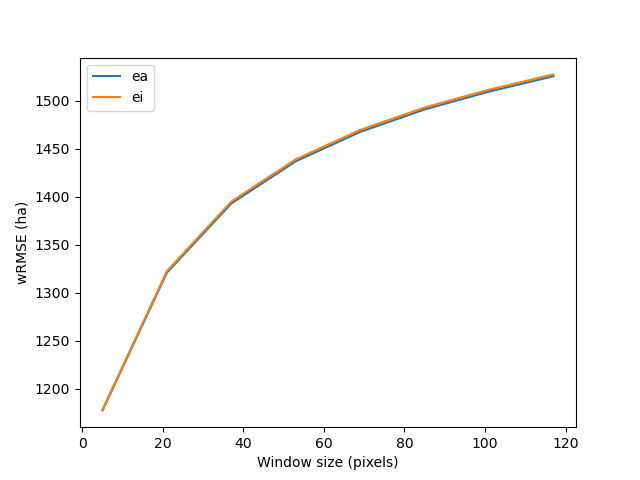
\includegraphics[width=\textwidth]{figs/map_comp.png}
\caption{\label{fig:org3ea48de}Prediction error as a function of window size.}
\end{figure}
\end{column}
\end{columns}
\end{frame}

\begin{frame}[label={sec:org775fcfe}]{Issues}
\begin{columns}
\begin{column}{0.5\columnwidth}
\begin{itemize}
\item Weak relationship between predictions and observations (high wRMSE).
\end{itemize}
\end{column}

\begin{column}{0.5\columnwidth}
\begin{figure}[htbp]
\centering
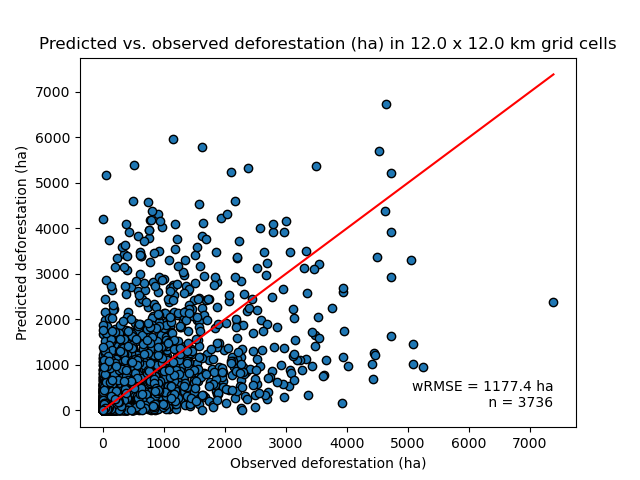
\includegraphics[width=\textwidth]{figs/pred_obs_kenya.png}
\caption{\label{fig:org81afec7}Predictions vs. observations for Kenya.}
\end{figure}
\end{column}
\end{columns}
\end{frame}

\begin{frame}[label={sec:org44f56a4},fragile]{Discussions with partners}
 \begin{itemize}
\item Cirad, FAO, IMPRESS, Verra and CBI.
\item To improve the methodology itself.
\item To test the \texttt{riskmapjnr} package and have feedbacks.
\item To increase computational speed on Sepal (use of GPU).
\end{itemize}
\end{frame}

\subsection{Alternative approach}
\label{sec:org1227862}

\begin{frame}[label={sec:org27500ae},fragile]{Alternative approach}
 \begin{itemize}
\item Comparison with the \texttt{forestatrisk} approach
\item Statistical model estimating the deforestation risk \(\theta\)
\item \(\theta\) = function(environmental variables + location)
\item Variables: distance to forest edge, roads, towns, protected areas
\end{itemize}

\vspace{0.5cm}
\begin{center}
\url{https://ecology.ghislainv.fr/forestatrisk/}
\end{center}
\end{frame}

% %%%%%%%%%%%%%%%%%%%%%%%%%%%%%%%%%%%%%%%%%%%%%%%%%%%%%%%%%%

{
  % Use background image
  \usebackgroundtemplate{%
    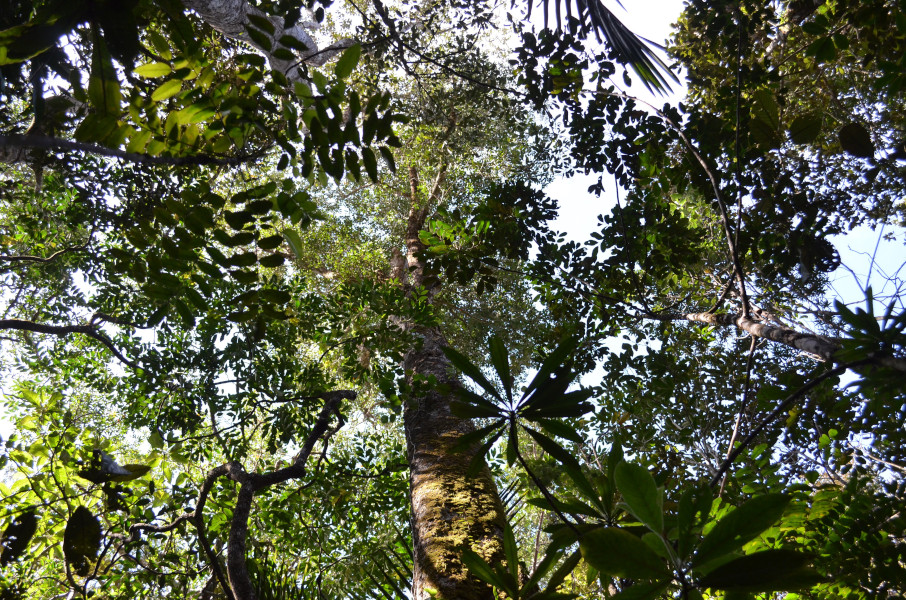
\includegraphics[keepaspectratio=true, height=\paperheight]{figs/Canopy-NC}
  }
  \setbeamertemplate{navigation symbols}{}
  % Remove shadow from block
  \setbeamertemplate{blocks}[rounded][shadow=false]
  \begin{frame}[plain]
  	\vspace*{\stretch{100}} 
    \begin{block}{}
      \begin{center}
        \ldots~Thank you for attention~\ldots \\
        \url{https://ecology.ghislainv.fr/presentations} \\
        
\includegraphics[width=0.45\textwidth]{figs/partners_logos}
      \end{center}
    \end{block}
  \end{frame}
}
\end{document}